%
% Copyright (c) 2017 Intel Corporation
%
% Permission is hereby granted, free of charge, to any person obtaining a copy
% of this software and associated documentation files (the "Software"), to
% deal in the Software without restriction, including without limitation the
% rights to use, copy, modify, merge, publish, distribute, sublicense, and/or
% sell copies of the Software, and to permit persons to whom the Software is
% furnished to do so, subject to the following conditions:
%
% The above copyright notice and this permission notice shall be included in
% all copies or substantial portions of the Software.
%
% THE SOFTWARE IS PROVIDED "AS IS", WITHOUT WARRANTY OF ANY KIND, EXPRESS OR
% IMPLIED, INCLUDING BUT NOT LIMITED TO THE WARRANTIES OF MERCHANTABILITY,
% FITNESS FOR A PARTICULAR PURPOSE AND NONINFRINGEMENT. IN NO EVENT SHALL THE
% AUTHORS OR COPYRIGHT HOLDERS BE LIABLE FOR ANY CLAIM, DAMAGES OR OTHER
% LIABILITY, WHETHER IN AN ACTION OF CONTRACT, TORT OR OTHERWISE, ARISING
% FROM, OUT OF OR IN CONNECTION WITH THE SOFTWARE OR THE USE OR OTHER DEALINGS
% IN THE SOFTWARE.
%

\newcommand{\repoTopPath}{../../..}
\newcommand{\commonPreamblePath}{\repoTopPath/common/latex/common_preamble.tex}
\input \commonPreamblePath

%----BEGIN TYPESETTING----------------------------------------------------------
\begin{document}
\sffamily

% create our own title area rather than \begin{titlepage} or \maketitle
\begin{center}
\let\savethefootnote\thefootnote
\let\thefootnote\relax\footnote{Cyclone, Intel, and Quartus are trademarks of Intel Corporation or its subsidiaries in the U.S. and/or other countries.}
\addtocounter{footnote}{-1}
\let\thefootnote\savethefootnote
\hspace{-1em}
\let\savethefootnote\thefootnote
\let\thefootnote\relax\footnote{Other names and brands may be claimed as the property of others.}
\addtocounter{footnote}{-1}
\let\thefootnote\savethefootnote
\hspace{-1em}
\LARGE{How to Program Your First FPGA Device}\\[1em]
\end{center}

\begin{flushleft}
\normalsize{PDF created: \today}\\
\normalsize{Validated using tools release: \TheToolsReleaseVersion}
\end{flushleft}

% make an entry in the PDF bookmarks for the TOC
\pdfbookmark[0]{Contents}{sumario_label}
% insert the default TOC format
\tableofcontents

%----NEW SECTION DEFINITION-----------------------------------------------------
\section*{Description}
% must manually add TOC reference for unnumbered section
\addcontentsline{toc}{section}{Description}
%----NEW SECTION DEFINITION-----------------------------------------------------

\begin{flushleft}
\noindent

This tutorial shows you how to create the hardware equivalent of \textquote{Hello World}: a blinking LED. This is a simple exercise to get you started using the Intel\textsuperscript{\textregistered} Quartus\textsuperscript{\textregistered} software for FPGA development.
\newline
\newline
You'll learn to compile Verilog\textsuperscript{*} code, make pin assignments, create timing constraints, and then program the FPGA to blink one of the eight green user LEDs on the board. You'll use a 50 MHz clock input (from the on-board oscillator) to drive a counter, and assign an LED to one of the counter output bits.
\newline
\newline
\textbf{Level:} beginner

\end{flushleft}

%----NEW SECTION DEFINITION-----------------------------------------------------
\section*{Materials}
% must manually add TOC reference for unnumbered section
\addcontentsline{toc}{section}{Materials}
%----NEW SECTION DEFINITION-----------------------------------------------------

%----NEW SUBSECTION DEFINITION-----------------------------------------------------
\subsection*{Hardware}
% must manually add TOC reference for unnumbered section
\addcontentsline{toc}{subsection}{Hardware}
%----NEW SUBSECTION DEFINITION-----------------------------------------------------

\begin{flushleft}

\begin{itemize}

\item Terasic DE10-Nano kit
\newline
\newline
The Terasic DE10-Nano development board, based on a Cyclone\textsuperscript{\textregistered} V SoC FPGA, provides a reconfigurable hardware design platform for makers, IoT developers and educators. You can buy the kit \href{https://www.terasic.com.tw/cgi-bin/page/archive.pl?Language=English&No=1046}{\underline{here}}.

\end{itemize}

\end{flushleft}

%----NEW SUBSECTION DEFINITION-----------------------------------------------------
\subsection*{Software}
% must manually add TOC reference for unnumbered section
\addcontentsline{toc}{subsection}{Software}
%----NEW SUBSECTION DEFINITION-----------------------------------------------------

\begin{flushleft}

\begin{itemize}

\item Intel Quartus Prime Software Suite Lite Edition
\newline
\newline
The FPGA design software used here is ideal for beginners as it's free to download and no license file is required. You can download the software \href{http://dl.altera.com/?edition=lite}{\underline{here}}.

\end{itemize}

\medskip

\begin{tcolorbox}[
	colback=MyMintedBGColor,
	colframe=MyMintedBGColor,
	]
\textbf{Note:} The installation files are large (several gigabytes) and can take a long time to download and install. To minimize download time and disk space required, we recommend you download only those items necessary for this exercise. When prompted which files to download, uncheck \textbf{Select All} and select only \textbf{Quartus Prime} and \textbf{Cyclone V device support} only.

\end{tcolorbox}

\begin{figure}[H]
\centering
% screen shots report a density of 37.8 PixelsPerCentimeter when actual resolution
% is more like 56 PixelsPerCentimeter, so the scaling factor for 1:1 is 0.675
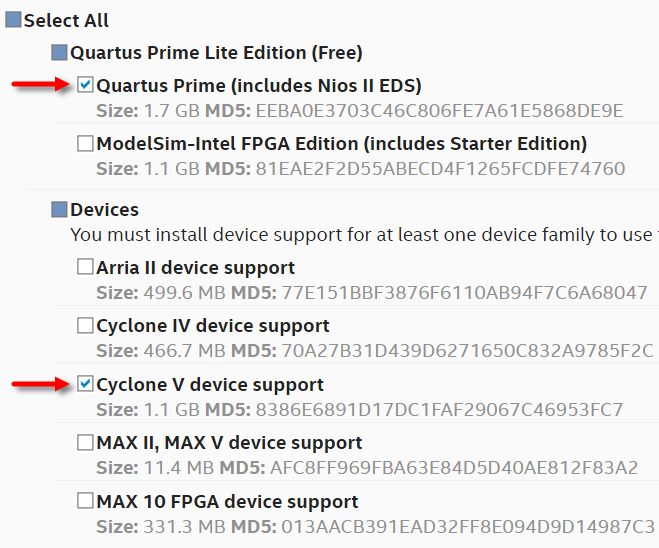
\includegraphics[scale=0.675]{01-quartus-tools}
\caption{Intel Quartus Prime Installation Options}
\label{fig:01-quartus-tools}
\end{figure}

Once you've downloaded and installed the Intel Quartus software, you're ready to get started creating a project!
\newline
\newline
\emph{Why is the Intel Quartus software download so big?} \hyperlink{side1}{\underline{Sidebar Topic}}
\newline

\begin{tcolorbox}[
	colback=MyMintedBGColor,
	colframe=MyMintedBGColor,
	]

\textbf{Note:} User experience may vary when using earlier or later versions of Intel Quartus software.  Screenshots in this document are based on the 16.1 release.

\end{tcolorbox}

\end{flushleft}

\newpage

%----NEW SECTION DEFINITION-----------------------------------------------------
\section*{Create the FPGA Design}
% must manually add TOC reference for unnumbered section
\addcontentsline{toc}{section}{Create the FPGA Design}
%----NEW SECTION DEFINITION-----------------------------------------------------

\begin{flushleft}

\begin{enumerate}[
	label=\textbf{Step \arabic*.},
	leftmargin=*,
	widest={00},
	align=left]

\item Create an Intel Quartus Software Project

\begin{enumerate}[
	label=\textbf{Step \arabic{enumi}\alph*.},
	leftmargin=*,
	align=left]

\item Open Intel Quartus Prime Software Suite Lite Edition.

\begin{figure}[H]
\centering
% screen shots report a density of 37.8 PixelsPerCentimeter when actual resolution
% is more like 56 PixelsPerCentimeter, so the scaling factor for 1:1 is 0.675
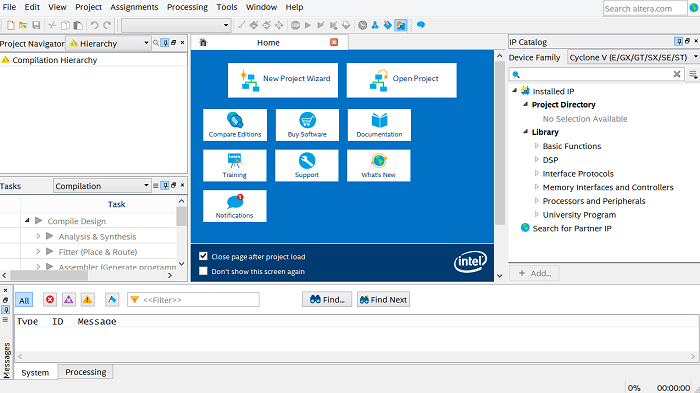
\includegraphics[scale=1.0]{02-quartus-window}
\caption{Intel Quartus Prime Software Window}
\label{fig:02-quartus-window}
\end{figure}

\item Open a \textbf{New Project Wizard}

\begin{figure}[H]
\centering
% screen shots report a density of 37.8 PixelsPerCentimeter when actual resolution
% is more like 56 PixelsPerCentimeter, so the scaling factor for 1:1 is 0.675
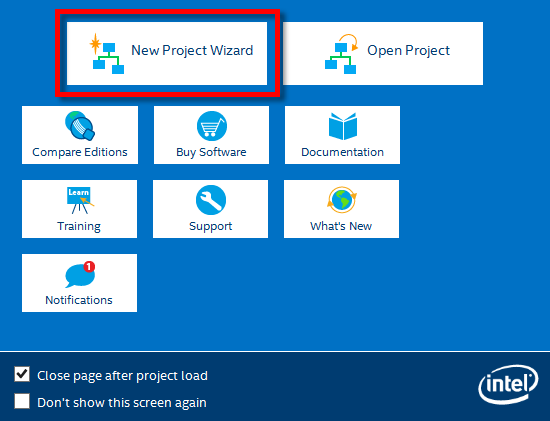
\includegraphics[scale=0.675]{03-new-project-button}
\caption{New Project Wizard Button}
\label{fig:03-new-project-button}
\end{figure}

\newpage

\item Select \textbf{Next}

\begin{figure}[H]
\centering
% screen shots report a density of 37.8 PixelsPerCentimeter when actual resolution
% is more like 56 PixelsPerCentimeter, so the scaling factor for 1:1 is 0.675
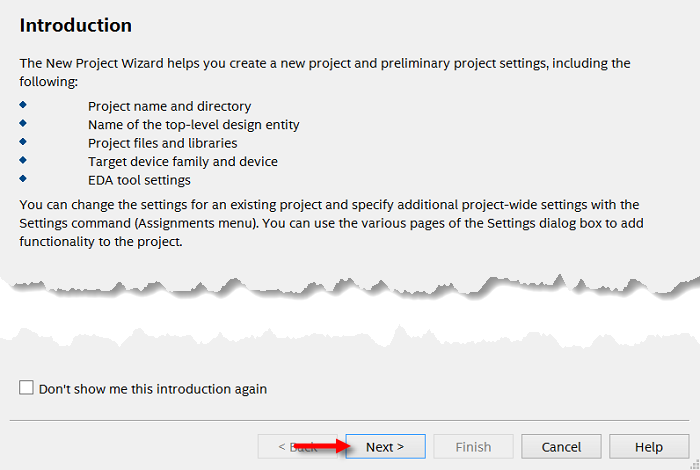
\includegraphics[scale=0.675]{04-introduction-next-button}
\caption{Introduction Dialog}
\label{fig:04-introduction-next-button}
\end{figure}

\item Directory, Name, Top-Level Entity
\newline
\newline
Choose a directory to put your project under. Let's name our project \textquote{blink} and place it under the IntelFPGA\_lite folder. Select \textbf{Next}.

\begin{figure}[H]
\centering
% screen shots report a density of 37.8 PixelsPerCentimeter when actual resolution
% is more like 56 PixelsPerCentimeter, so the scaling factor for 1:1 is 0.675
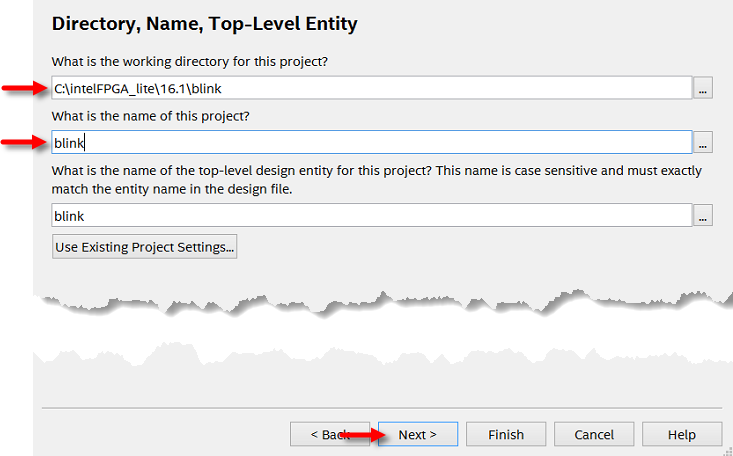
\includegraphics[scale=0.675]{05-project-location-details}
\caption{Project Location Details}
\label{fig:05-project-location-details}
\end{figure}

When prompted to create the directory, choose \textbf{Yes}.

\begin{figure}[H]
\centering
% screen shots report a density of 37.8 PixelsPerCentimeter when actual resolution
% is more like 56 PixelsPerCentimeter, so the scaling factor for 1:1 is 0.675
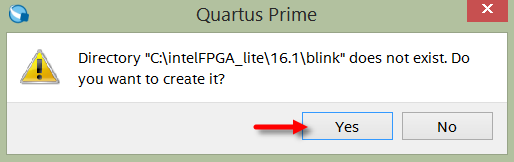
\includegraphics[scale=0.675]{06-create-directory-dialog}
\caption{Create Directory Dialog}
\label{fig:06-create-directory-dialog}
\end{figure}

This project directory is convenient for an example tutorial, but isn't what we would recommend for future projects.
\newline
\emph{Where should I put my future project files?} \hyperlink{side10}{\underline{Sidebar Topic}}
\newline

\item Project Type
\newline
\newline
Select \textbf{Empty Project}, and then click \textbf{Next}.

\begin{figure}[H]
\centering
% screen shots report a density of 37.8 PixelsPerCentimeter when actual resolution
% is more like 56 PixelsPerCentimeter, so the scaling factor for 1:1 is 0.675
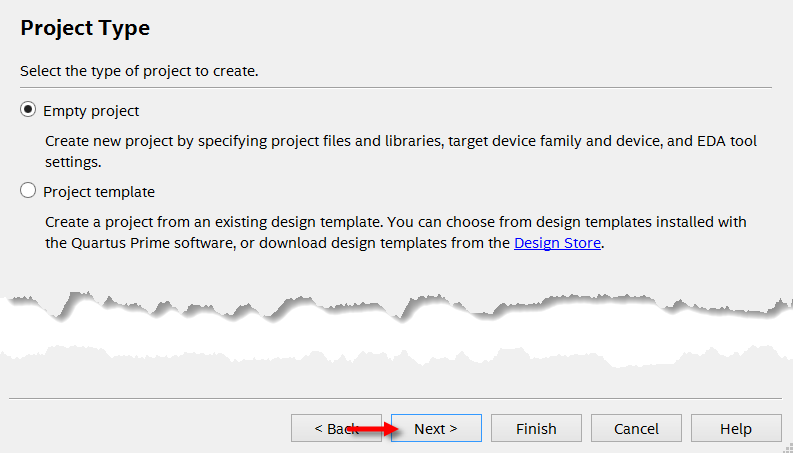
\includegraphics[scale=0.675]{07-project-type-dialog}
\caption{Project Type Dialog}
\label{fig:07-project-type-dialog}
\end{figure}

\item Add Files
\newline
\newline
You won't be adding any files here. Click \textbf{Next}.

\begin{figure}[H]
\centering
% screen shots report a density of 37.8 PixelsPerCentimeter when actual resolution
% is more like 56 PixelsPerCentimeter, so the scaling factor for 1:1 is 0.675
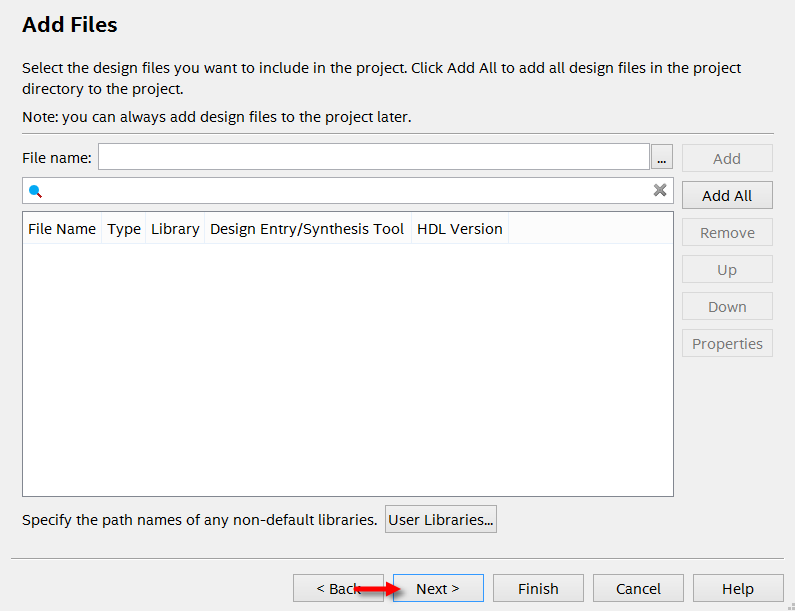
\includegraphics[scale=0.675]{08-add-files-dialog}
\caption{Add Files Dialog}
\label{fig:08-add-files-dialog}
\end{figure}

\newpage

\item Family, Device, and Board Settings

\begin{tcolorbox}[
	colback=MyMintedBGColor,
	colframe=MyMintedBGColor,
	]
\textbf{Note:} You may need to expand the window to view more device names
\end{tcolorbox}

Select the following:

\begin{itemize}
\item \emph{Family}: \textbf{Cyclone V}
\item \emph{Device}: \textbf{Cyclone V SE Base}
\item \emph{Device name}: \textbf{5CSEBA6U23I7}
\end{itemize}

\begin{tcolorbox}[
	colback=MyMintedBGColor,
	colframe=MyMintedBGColor,
	]
\textbf{Note}: To select the specific device you will need to click the up/down arrows to scroll through the list of supported devices until you find 5CSEBA6U23I7. Alternatively, you can enter the device name in the \textbf{Name filter} box to narrow down the list of devices. You may also need to expand the \textbf{Name} field to see the full device name.
\end{tcolorbox}

\begin{figure}[H]
\centering
% screen shots report a density of 37.8 PixelsPerCentimeter when actual resolution
% is more like 56 PixelsPerCentimeter, so the scaling factor for 1:1 is 0.675
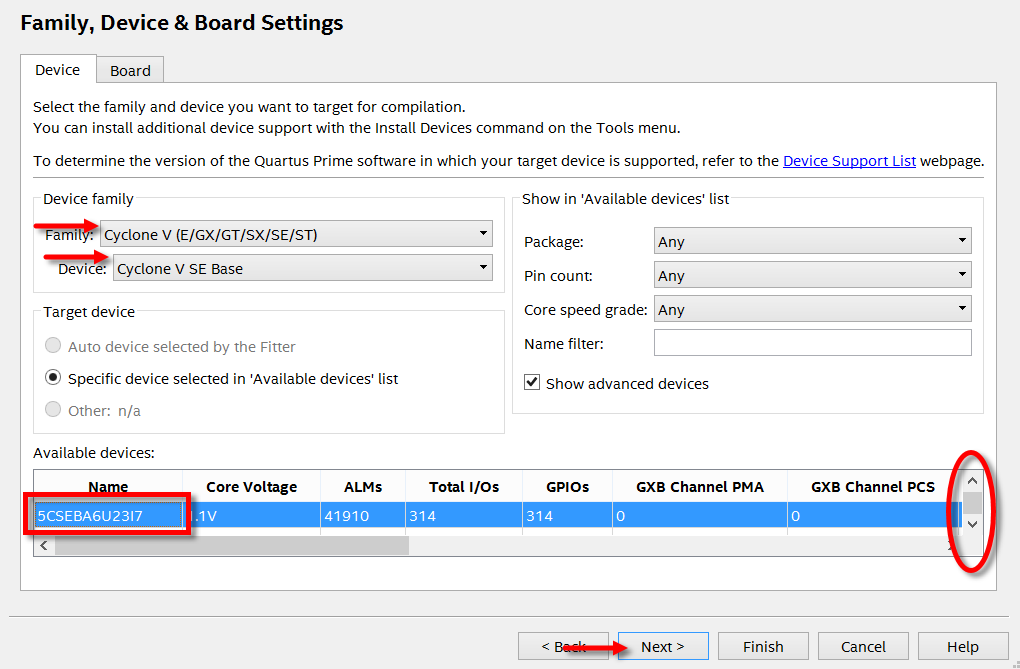
\includegraphics[scale=0.675]{09-family-device-dialog}
\caption{Family and Device Dialog}
\label{fig:09-family-device-dialog}
\end{figure}

Click \textbf{Next}.
\newline

\newpage

\item EDA Tool Settings
\newline
\newline
We will be using the default EDA tools and settings so there are no changes to be made. Click~\textbf{Next}.

\begin{figure}[H]
\centering
% screen shots report a density of 37.8 PixelsPerCentimeter when actual resolution
% is more like 56 PixelsPerCentimeter, so the scaling factor for 1:1 is 0.675
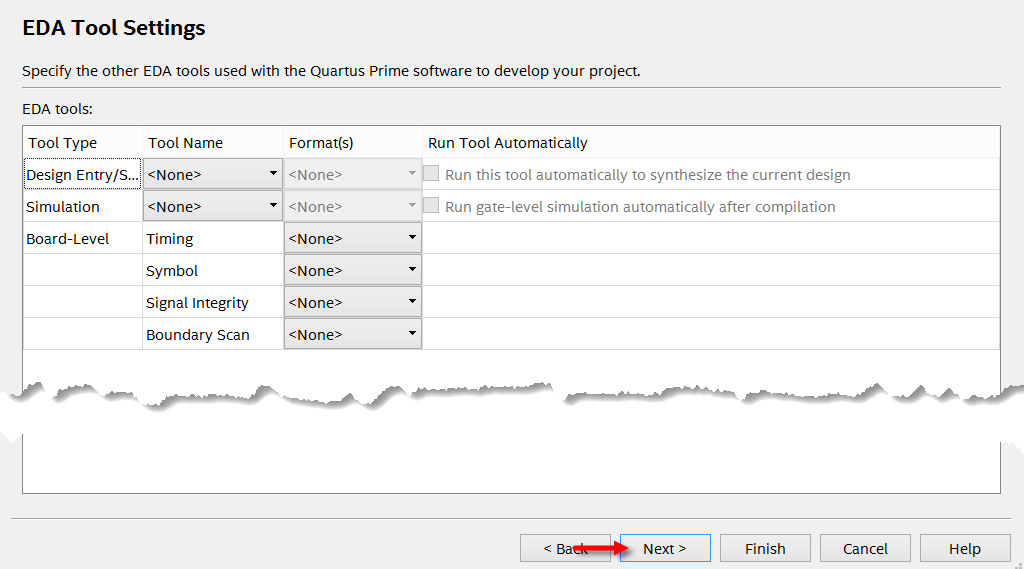
\includegraphics[scale=0.675]{10-eda-tool-dialog}
\caption{EDA Tools Dialog}
\label{fig:10-eda-tool-dialog}
\end{figure}

\item Summary
\newline
\newline
Click \textbf{Finish}.

\begin{figure}[H]
\centering
% screen shots report a density of 37.8 PixelsPerCentimeter when actual resolution
% is more like 56 PixelsPerCentimeter, so the scaling factor for 1:1 is 0.675
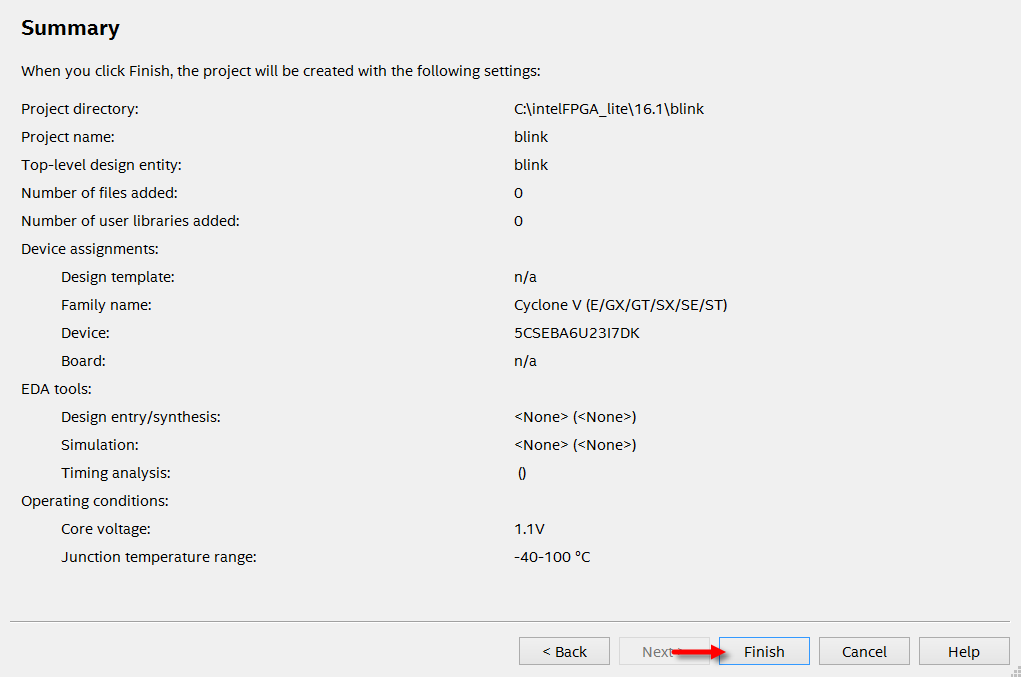
\includegraphics[scale=0.675]{11-summary-dialog}
\caption{Summary Dialog}
\label{fig:11-summary-dialog}
\end{figure}

\newpage

The following screen displays.

\begin{figure}[H]
\centering
% screen shots report a density of 37.8 PixelsPerCentimeter when actual resolution
% is more like 56 PixelsPerCentimeter, so the scaling factor for 1:1 is 0.675
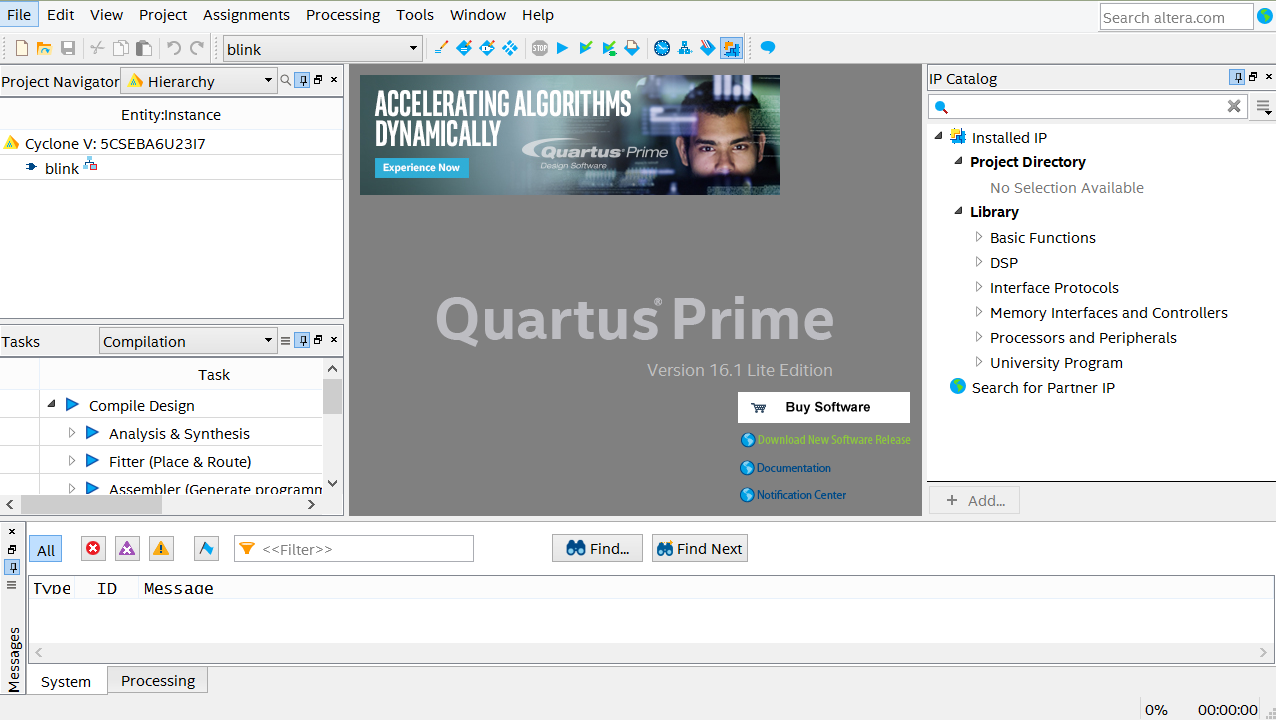
\includegraphics[scale=0.500]{12-project-window}
\caption{Your First Project Window}
\label{fig:12-project-window}
\end{figure}

\end{enumerate}

\item Create an HDL File
\newline
\newline
\textbf{Hardware Description Language (HDL)}
\newline
\newline
We use Verilog as the HDL. If you are familiar with the C programming language but new to programming in an HDL, Verilog is similar to C.

\begin{enumerate}[
	label=\textbf{Step \arabic{enumi}\alph*.},
	leftmargin=*,
	align=left]

\item Navigate to the File tab (main window), and then select \textbf{New}.

\begin{figure}[H]
\centering
% screen shots report a density of 37.8 PixelsPerCentimeter when actual resolution
% is more like 56 PixelsPerCentimeter, so the scaling factor for 1:1 is 0.675
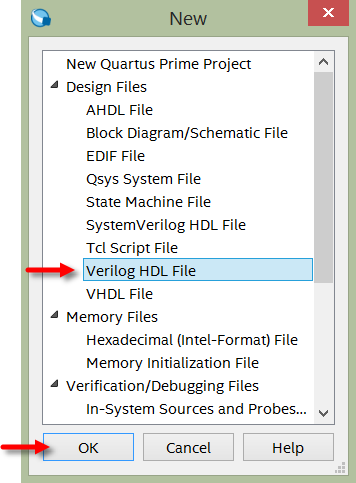
\includegraphics[scale=0.675]{13-verilog-file-selection}
\caption{Select New Verilog HDL File}
\label{fig:13-verilog-file-selection}
\end{figure}

Select \textbf{Verilog HDL File}, and then click \textbf{OK}.

\item Choose \textbf{File} > \textbf{Save As}. Choose \textquote{blink} for the file name. This is your top-level file name (blink.v). Click \textbf{Save}.

\begin{figure}[H]
\centering
% screen shots report a density of 37.8 PixelsPerCentimeter when actual resolution
% is more like 56 PixelsPerCentimeter, so the scaling factor for 1:1 is 0.675
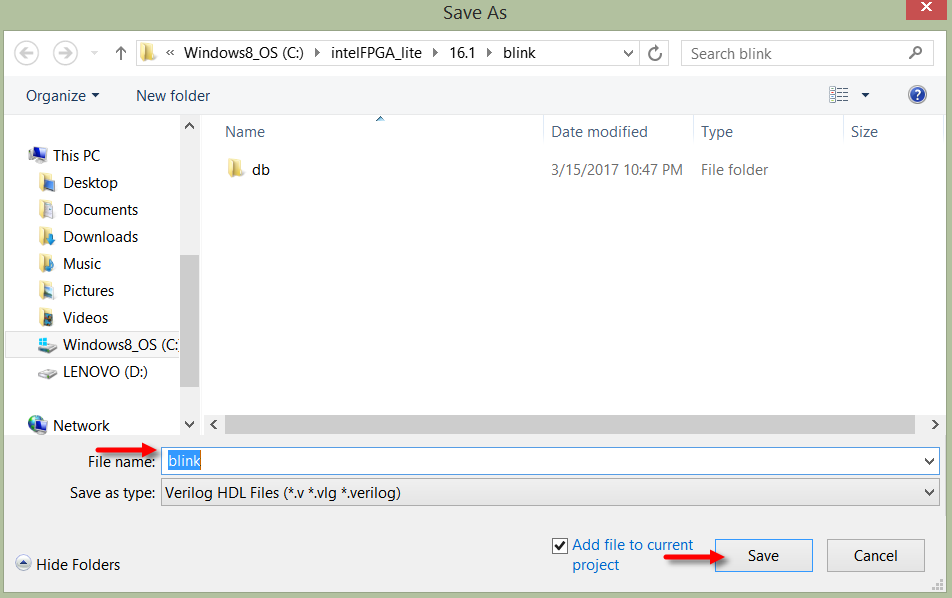
\includegraphics[scale=0.675]{14-verilog-file-naming}
\caption{Saving Verilog HDL File}
\label{fig:14-verilog-file-naming}
\end{figure}

\end{enumerate}

\item Create a Verilog Module

\begin{enumerate}[
	label=\textbf{Step \arabic{enumi}\alph*.},
	leftmargin=*,
	align=left]

%\item Extract this Verilog code from the PDF file and paste it into the blink.v window, and then save the file.
%\newline
%\newline
%Extract this Verilog HDL file from the PDF file.  Right click on the PDF attachment link and your PDF reader should present a pop-up menu with an option to save the attachment to your local file system.  Optionally, you may be able to double click on the PDF attachment link and your system may open it in a text editor.
%\newline
%\newline
%Extract PDF Attachment: \textattachfile[
%        color=0.0 0.678 0.937,
%        mimetype=text/plain,
%        description={Verilog Source File: blink.v}
%]{../../hdl_src/blink.v}{\textbf{blink.v}}

\item Download this Verilog code from the GitHub\textsuperscript{*} repository and paste it into the blink.v window, and then save the file.
\newline
\newline
Download the blink.v file \href{\TheRawURL/MyFirstFPGA/hdl_src/blink.v}{\underline{here}}.
\newline
If you wish to view the blink.v file in the GitHub repo you can look \href{\TheBlobURL/MyFirstFPGA/hdl_src/blink.v}{\underline{here}}.

\inputminted[
        bgcolor=MyMintedBGColor,
        linenos,
        fontsize=\footnotesize
]{verilog}{../../hdl_src/blink.v}

\begin{figure}[H]
\centering
% screen shots report a density of 37.8 PixelsPerCentimeter when actual resolution
% is more like 56 PixelsPerCentimeter, so the scaling factor for 1:1 is 0.675
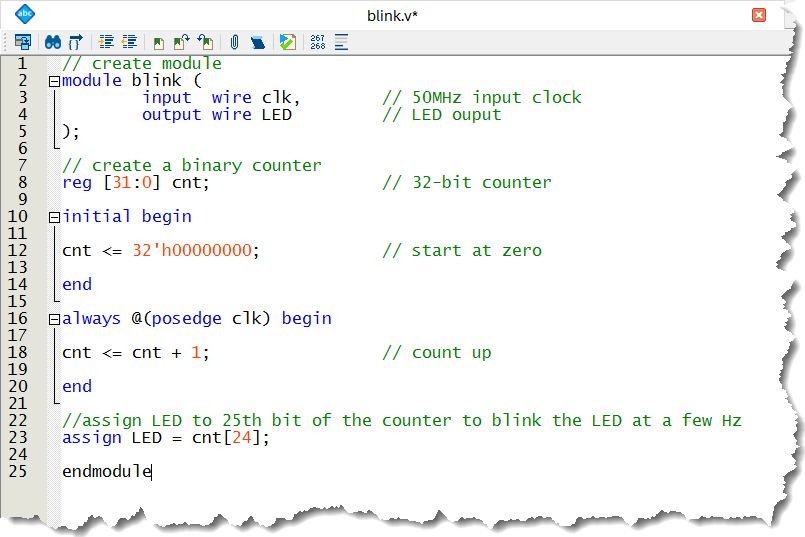
\includegraphics[scale=0.675]{15-verilog-code-editor}
\caption{Verilog HDL Pasted in Editor}
\label{fig:15-verilog-code-editor}
\end{figure}

\newpage

\item Analysis \& Synthesis
\newline
\newline
Right click on \textbf{Analysis and Synthesis}, and then click \textbf{Start} to perform a syntax check and synthesis of the Verilog code.  If you do not see the \textbf{Tasks} pane in your view, go to the \textbf{View} menu and select \textbf{Utility Windows} and then select \textbf{Tasks}.

\begin{figure}[H]
\centering
% screen shots report a density of 37.8 PixelsPerCentimeter when actual resolution
% is more like 56 PixelsPerCentimeter, so the scaling factor for 1:1 is 0.675
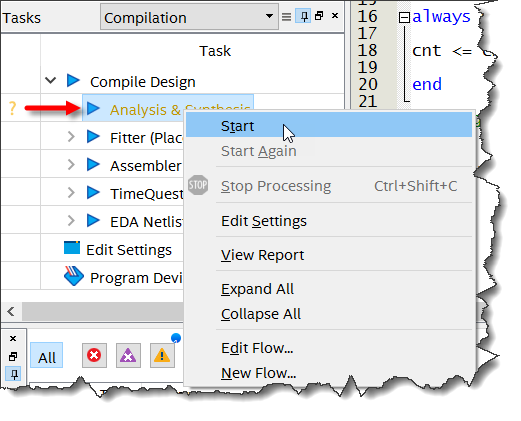
\includegraphics[scale=0.675]{16-start-analysis}
\caption{Start Analysis and Synthesis}
\label{fig:16-start-analysis}
\end{figure}

\emph{What happens during analysis and synthesis?} \hyperlink{side2}{\underline{Sidebar Topic}}
\newline
\newline
If the process completes successfully, a green check mark displays next to Analysis \& Synthesis. If you get an error, check your syntax and make sure it matches exactly the code block provided above.

\begin{figure}[H]
\centering
% screen shots report a density of 37.8 PixelsPerCentimeter when actual resolution
% is more like 56 PixelsPerCentimeter, so the scaling factor for 1:1 is 0.675
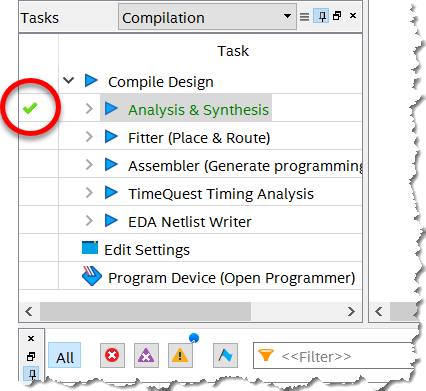
\includegraphics[scale=0.675]{17-analysis-complete}
\caption{Analysis Complete}
\label{fig:17-analysis-complete}
\end{figure}

\end{enumerate}

\newpage

\item Choose Pin Assignments

\begin{enumerate}[
	label=\textbf{Step \arabic{enumi}\alph*.},
	leftmargin=*,
	align=left]

\item In the top navigation bar, select \textbf{Assignments} > \textbf{Pin Planner}.

\begin{figure}[H]
\centering
% screen shots report a density of 37.8 PixelsPerCentimeter when actual resolution
% is more like 56 PixelsPerCentimeter, so the scaling factor for 1:1 is 0.675
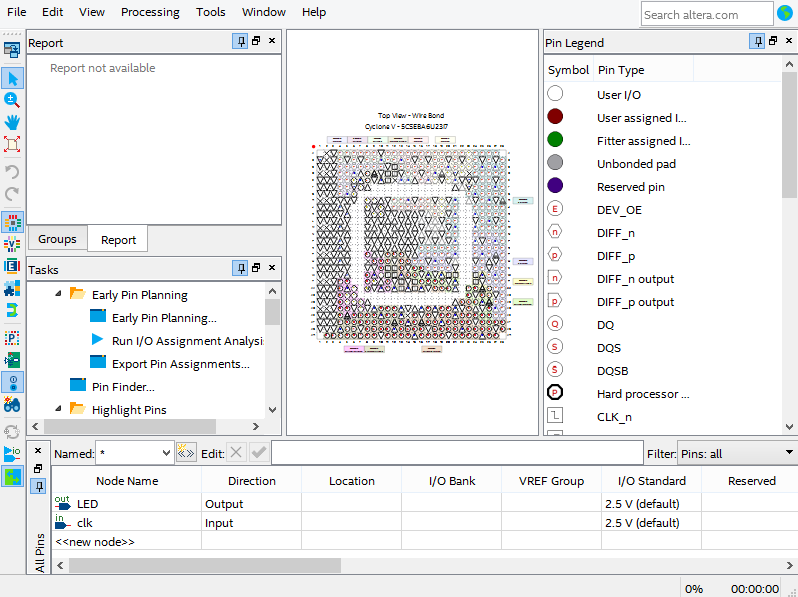
\includegraphics[scale=0.750]{18-pin-planner-one}
\caption{Pin Planner Window}
\label{fig:18-pin-planner-one}
\end{figure}

Notice that the input (clk) and output (LED) are listed under \textbf{Node Name}. This is because you ran the Analysis \& Synthesis.

\item One at a time, click to highlight the \textbf{Location} column for each pin, then type the pin location for the LED and clk signals as shown below. The rest of the columns will auto populate with data (some with default values that we'll modify in the next step).

\begin{center}
\begin{tabular}{ |c|c| }
\hline
Node Name & Location \\
\hline
LED & PIN\_W15 \\
clk & PIN\_V11 \\
\hline
\end{tabular}
\end{center}

\begin{figure}[H]
\centering
% screen shots report a density of 37.8 PixelsPerCentimeter when actual resolution
% is more like 56 PixelsPerCentimeter, so the scaling factor for 1:1 is 0.675
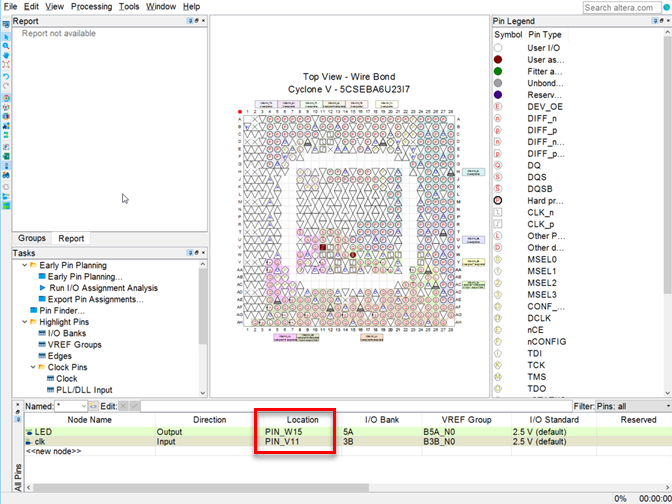
\includegraphics[scale=1.0]{19-pin-planner-locations}
\caption{Pin Planner Locations Set}
\label{fig:19-pin-planner-locations}
\end{figure}

You also need to change the \textbf{I/O standard}, \textbf{Current Strength} and \textbf{Slew Rate} columns from their default settings to the values shown below:

\begin{center}
\begin{tabular}{ |c|c|c|c|c| }
\hline
Node Name & Location & I/O Standard & Current Strength & Slew Rate\\
\hline
LED & PIN\_W15 & 3.3-V LVTTL & 16ma & 1 \\
clk & PIN\_V11 & 3.3-V LVTTL & 16ma &  \\
\hline
\end{tabular}
\end{center}

\item To change the \textbf{I/O standard}, double click each cell and a pull-down menu will appear. Click the down arrow icon and scroll to the desired value. Change the I/O standard from the default 2.5V to \textbf{3.3-V LVTTL}.

\item The Current Strength will by default read 16ma(default) and we need to select 16ma. If we don't specifically set them, then we get warning messages in our compilation. Set \textbf{Current Strength} to \textbf{16ma} for both input (clk) and output (LED).

\item Next change \textbf{Slew Rate} for the LED output from 1(default) to \textbf{1(fastest)}. You don't need to set a Slew Rate for the clk. Leave that blank.

\begin{figure}[H]
\centering
% screen shots report a density of 37.8 PixelsPerCentimeter when actual resolution
% is more like 56 PixelsPerCentimeter, so the scaling factor for 1:1 is 0.675
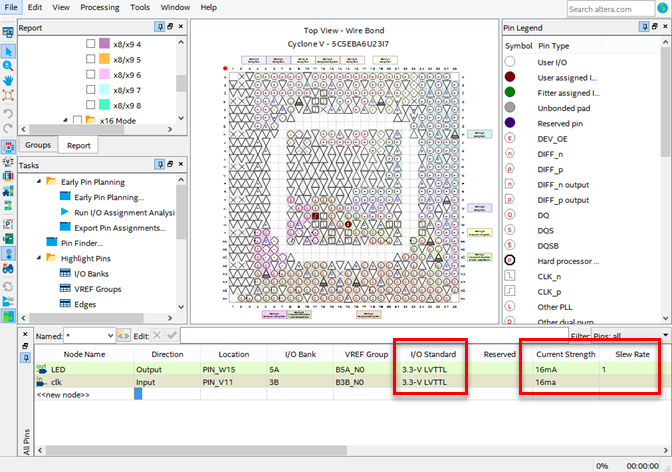
\includegraphics[scale=1.0]{20-pin-planner-io-cs}
\caption{Pin Planner All Set}
\label{fig:20-pin-planner-io-cs}
\end{figure}

\item Close the Pin Planner.  The changes that you make in the Pin Planner are saved automatically.

\end{enumerate}

\item Create an SDC File
\newline
\newline
Before you compile the Verilog code, you need to provide timing constraints for the design. You'll create an SDC (Synopsis Design Constraints) file that contains commands to let the Intel Quartus software know how to close timing on the design. Without it, you will get warning messages in the compile flow because the Intel Quartus software has no idea how to close timing on the design.

\begin{enumerate}[
	label=\textbf{Step \arabic{enumi}\alph*.},
	leftmargin=*,
	align=left]

%\item To create a blink.sdc and add it to the blink project directory, do the following.
%\newline
%\newline
%Extract this SDC file from the PDF file.  Right click on the PDF attachment link and your PDF reader should present a pop-up menu with an option to save the attachment to your local file system.
%\newline
%\newline
%Extract PDF Attachment: \textattachfile[
%        color=0.0 0.678 0.937,
%        mimetype=text/plain,
%        description={SDC Source File: blink.sdc}
%]{../../hdl_src/blink.sdc}{\textbf{blink.sdc}}

\item To create a blink.sdc and add it to the blink project directory, do the following.
\newline
\newline
Download the blink.sdc file \href{\TheRawURL/MyFirstFPGA/hdl_src/blink.sdc}{\underline{here}}.
\newline
If you wish to view the blink.sdc file in the GitHub repo you can look \href{\TheBlobURL/MyFirstFPGA/hdl_src/blink.sdc}{\underline{here}}.

\inputminted[
        bgcolor=MyMintedBGColor,
        linenos,
        fontsize=\footnotesize
]{tcl}{../../hdl_src/blink.sdc}

\item Now save the file as \textquote{blink.sdc}. Place it in the blink project directory - the same directory where our Verilog file (.v file extension) lives.
\newline
\emph{What is an SDC file, and why do I need one?} \hyperlink{side3}{\underline{Sidebar Topic}}

\begin{figure}[H]
\centering
% screen shots report a density of 37.8 PixelsPerCentimeter when actual resolution
% is more like 56 PixelsPerCentimeter, so the scaling factor for 1:1 is 0.675
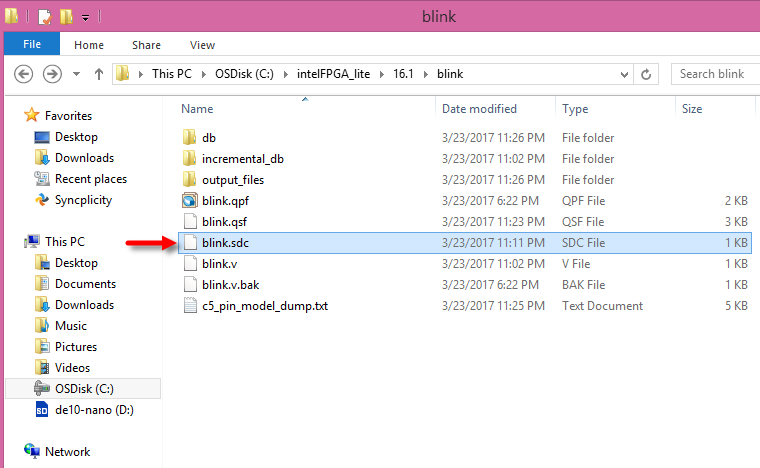
\includegraphics[scale=1.0]{21-sdc-file-location}
\caption{SDC File Location}
\label{fig:21-sdc-file-location}
\end{figure}

\item Now you need to add this SDC this file to the Intel Quartus software project.  Select the \textbf{Project} menu and then \textbf{Add/Remove Files in Project...}.  In the \textbf{Settings} dialog that appears, click the browse \textbf{...} button to the right of the \textbf{File name} text box.  This will bring up a file browser dialog.  Change the \textbf{Files of type} option to \textbf{Script Files} or \textbf{All Files} so that the \textquote{blink.sdc} file is displayed.  Select the \textquote{blink.sdc} file and click the \textbf{Open} button to close the dialog.  At this point the \textquote{blink.sdc} file should appear in the project files list and you can click the \textbf{OK} button to close the \textbf{Settings} dialog.

\end{enumerate}

\newpage

\item Compile the Verilog Code

\begin{enumerate}[
	label=\textbf{Step \arabic{enumi}\alph*.},
	leftmargin=*,
	align=left]

\item Right click on \textbf{Compile Design}, and then click \textbf{Start}. The tools will then synthesize, place and route, assemble and perform timing analysis on the design.  Because there are only a handful of code lines, the compilation should only take a couple of minutes to complete.
\newline
\newline
\emph{What happens during the fitter (place \& route)?} \hyperlink{side4}{\underline{Sidebar Topic}}
\newline
\newline
\emph{What happens during the assembler?} \hyperlink{side5}{\underline{Sidebar Topic}}
\newline
\newline
\emph{What is timing analysis?} \hyperlink{side6}{\underline{Sidebar Topic}}

\begin{figure}[H]
\centering
% screen shots report a density of 37.8 PixelsPerCentimeter when actual resolution
% is more like 56 PixelsPerCentimeter, so the scaling factor for 1:1 is 0.675
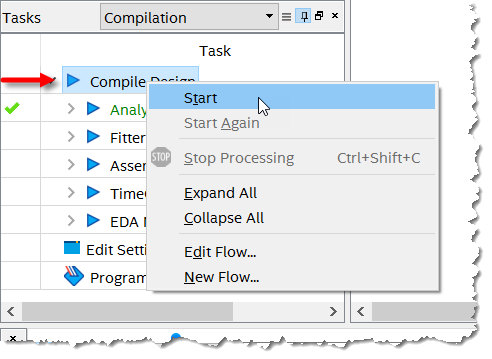
\includegraphics[scale=0.675]{22-compile-design}
\caption{Compile Design}
\label{fig:22-compile-design}
\end{figure}

After compilation is complete you will see a summary report like the one below.

\begin{figure}[H]
\centering
% screen shots report a density of 37.8 PixelsPerCentimeter when actual resolution
% is more like 56 PixelsPerCentimeter, so the scaling factor for 1:1 is 0.675
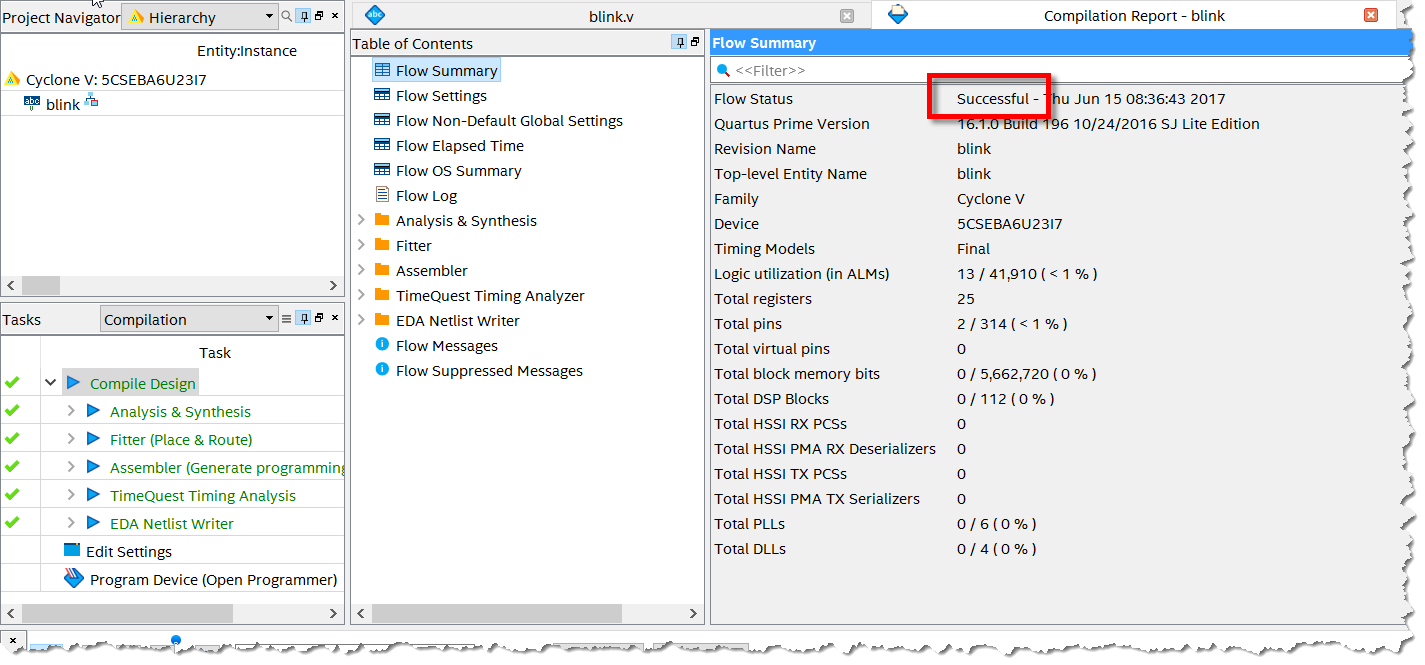
\includegraphics[scale=0.600]{23-compile-summary}
\caption{Compile Summary}
\label{fig:23-compile-summary}
\end{figure}

After you compile the Verilog code, you can program the FPGA.

\end{enumerate}

\newpage

\item Program the FPGA
\newline
\newline
The final step is to program the FPGA. Before we do that, be sure to remove the SD Card from the board.
\newline
\newline
\emph{Why should I remove the SD Card?} \hyperlink{side7}{\underline{Sidebar Topic}}
\newline
\newline
To program the FPGA, you need to connect the board to your computer via the USB Blaster II port.

\begin{enumerate}[
	label=\textbf{Step \arabic{enumi}\alph*.},
	leftmargin=*,
	align=left]

\item Connect the board to your computer via the USB Blaster II port. Use the USB cable (mini-b connector) that came with the Terasic DE10-Nano kit. Insert the mini-b connector into the USB Blaster II port (J13) on the Terasic DE10-Nano board and the Type-A end into a standard USB port on your host computer.

\item Connect the board to power and verify there is a blue LED lit near the J13 USB Blaster II port.

\item Right click to open \textbf{Program Device}.

\begin{figure}[H]
\centering
% screen shots report a density of 37.8 PixelsPerCentimeter when actual resolution
% is more like 56 PixelsPerCentimeter, so the scaling factor for 1:1 is 0.675
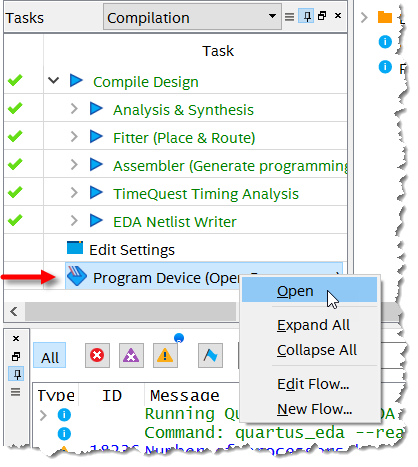
\includegraphics[scale=0.675]{24-open-programmer}
\caption{Open Intel Quartus Software Programmer}
\label{fig:24-open-programmer}
\end{figure}

\item Hardware Setup
\newline
\newline
Select \textbf{Hardware Setup}.

\begin{figure}[H]
\centering
% screen shots report a density of 37.8 PixelsPerCentimeter when actual resolution
% is more like 56 PixelsPerCentimeter, so the scaling factor for 1:1 is 0.675
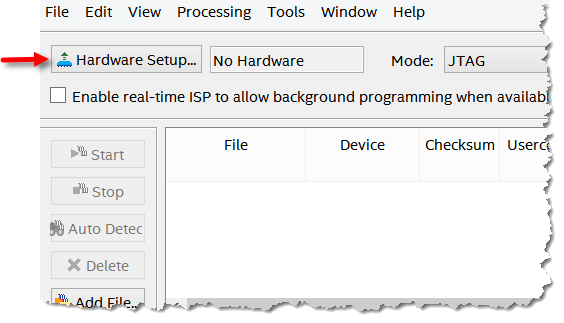
\includegraphics[scale=0.675]{25-hardware-setup}
\caption{Hardware Setup}
\label{fig:25-hardware-setup}
\end{figure}

\newpage

Under the drop down for \textbf{Currently selected hardware}, choose \textbf{DE-SoC}, then click \textbf{Close}.

\begin{figure}[H]
\centering
% screen shots report a density of 37.8 PixelsPerCentimeter when actual resolution
% is more like 56 PixelsPerCentimeter, so the scaling factor for 1:1 is 0.675
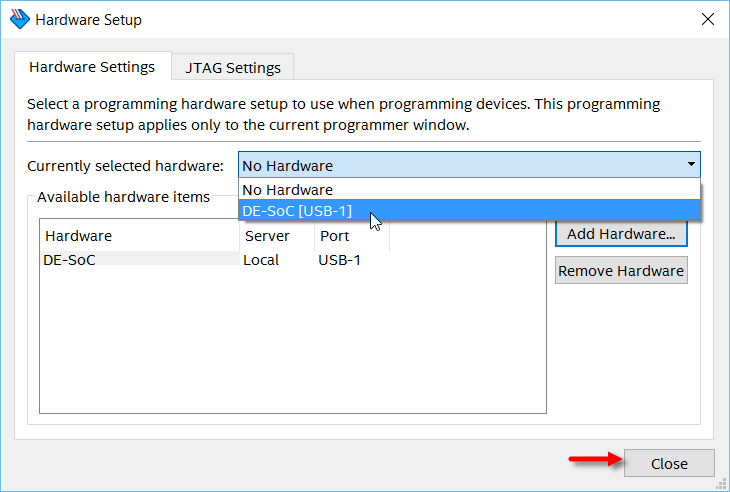
\includegraphics[scale=0.675]{26-cable-selection}
\caption{Cable Selection}
\label{fig:26-cable-selection}
\end{figure}

\item Click \textbf{Auto Detect} to identify the JTAG chain on the board.

\begin{figure}[H]
\centering
% screen shots report a density of 37.8 PixelsPerCentimeter when actual resolution
% is more like 56 PixelsPerCentimeter, so the scaling factor for 1:1 is 0.675
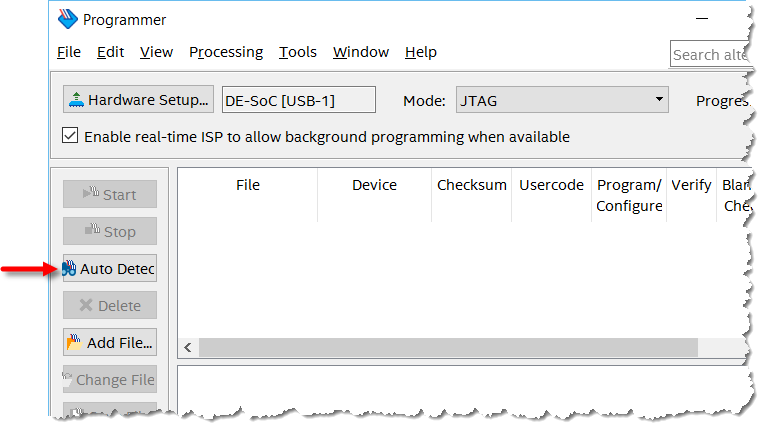
\includegraphics[scale=0.675]{27-auto-detect}
\caption{Auto Detect}
\label{fig:27-auto-detect}
\end{figure}

\newpage

Select the device \textbf{5CSEBA6}. This is the FPGA device.

\begin{figure}[H]
\centering
% screen shots report a density of 37.8 PixelsPerCentimeter when actual resolution
% is more like 56 PixelsPerCentimeter, so the scaling factor for 1:1 is 0.675
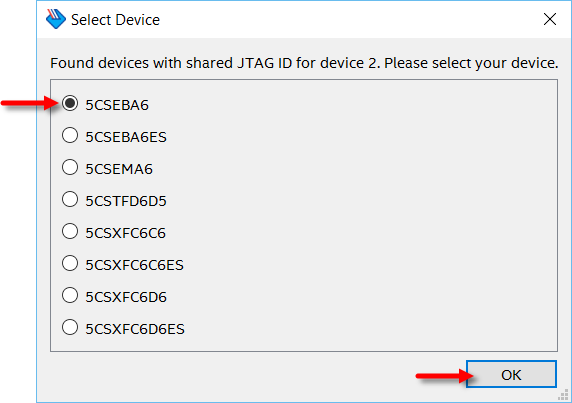
\includegraphics[scale=0.675]{28-device-selection}
\caption{Device Selection}
\label{fig:28-device-selection}
\end{figure}

\item Add the .sof file.
\newline
\newline
Right click on the \textbf{File} column for the \textbf{5CSEBA6} device and select \textbf{Change File}.
\newline
\newline
\emph{Why are there two devices found in the JTAG chain?} \hyperlink{side8}{\underline{Sidebar Topic}}

\begin{figure}[H]
\centering
% screen shots report a density of 37.8 PixelsPerCentimeter when actual resolution
% is more like 56 PixelsPerCentimeter, so the scaling factor for 1:1 is 0.675
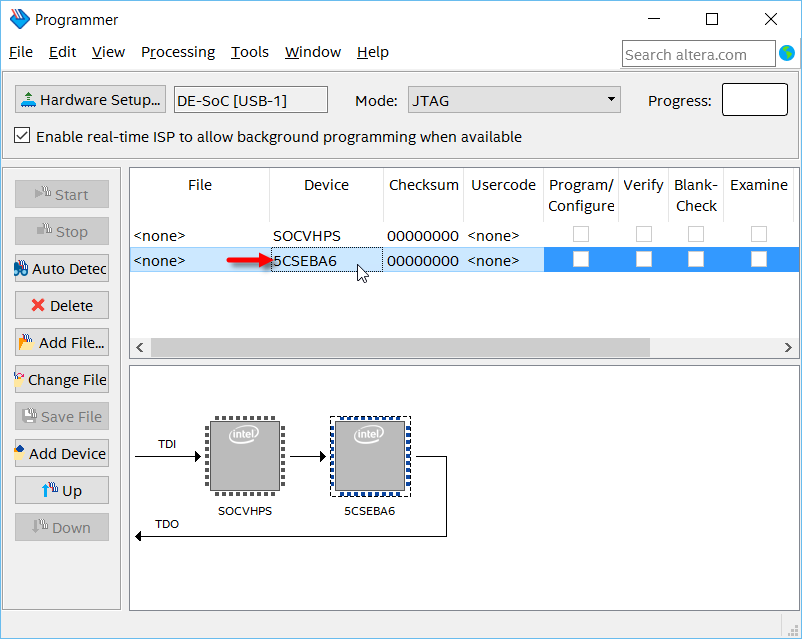
\includegraphics[scale=0.675]{29-change-file}
\caption{Change File}
\label{fig:29-change-file}
\end{figure}

\newpage

\item Navigate to the \emph{output\_files} folder, select \textbf{blink.sof}, and then click \textbf{Open}.

\begin{figure}[H]
\centering
% screen shots report a density of 37.8 PixelsPerCentimeter when actual resolution
% is more like 56 PixelsPerCentimeter, so the scaling factor for 1:1 is 0.675
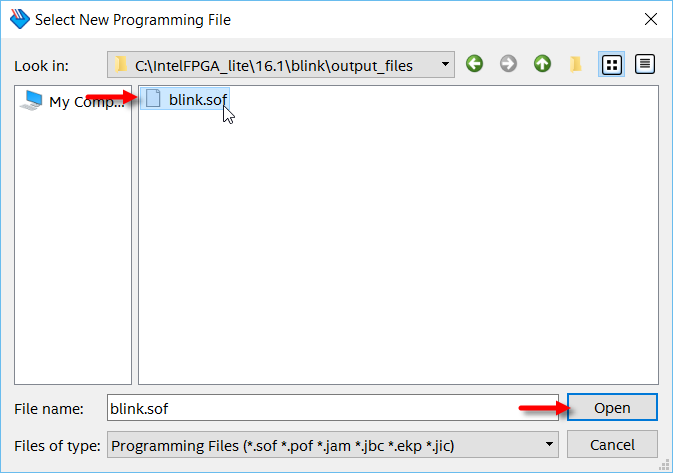
\includegraphics[scale=0.675]{30-sof-file}
\caption{Select SOF File}
\label{fig:30-sof-file}
\end{figure}

Here, \textbf{blink.sof} is your programming file. SRAM Object Files (.sof files) are binary files containing data for configuring SRAM-based devices, our FPGA is based on SRAM.  The Intel Quartus software Program Device (also called the Quartus Programmer) looks into the SOF file and gets the programming bit stream for the device.
\newline

\item Check the \textbf{Program/Configure} column, and then click \textbf{Start}.

\begin{figure}[H]
\centering
% screen shots report a density of 37.8 PixelsPerCentimeter when actual resolution
% is more like 56 PixelsPerCentimeter, so the scaling factor for 1:1 is 0.675
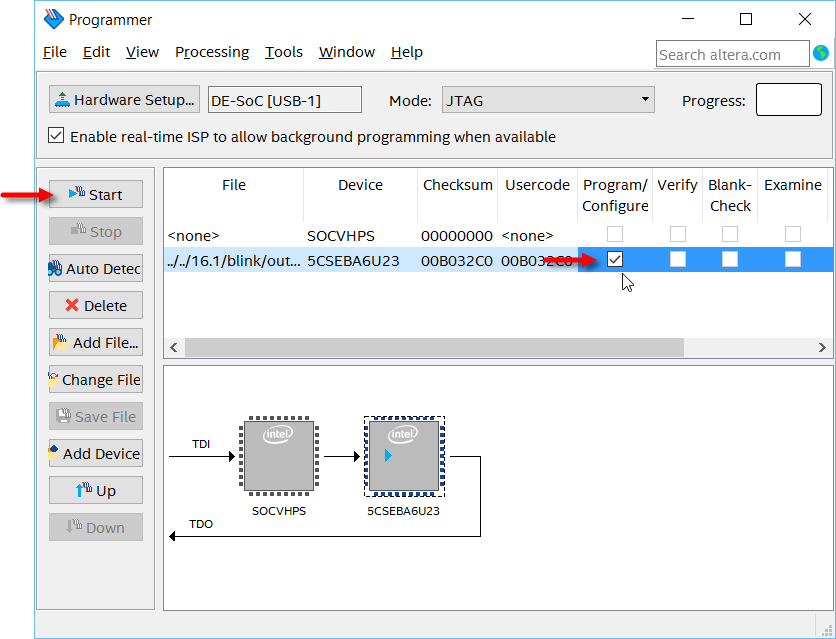
\includegraphics[scale=0.675]{31-start-programmer}
\caption{Start Programming}
\label{fig:31-start-programmer}
\end{figure}

\end{enumerate}

\newpage

\item Observe the blinking LED
\newline
\newline
If your progress bar is 100\% (Successful), watch LED[0] blink.

\begin{figure}[H]
\centering
% screen shots report a density of 37.8 PixelsPerCentimeter when actual resolution
% is more like 56 PixelsPerCentimeter, so the scaling factor for 1:1 is 0.675
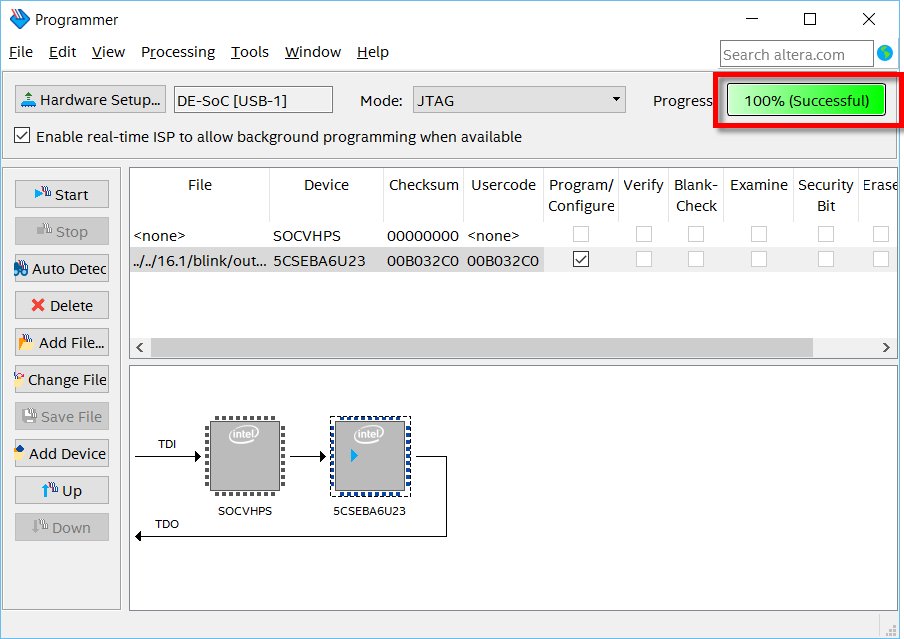
\includegraphics[scale=0.675]{32-programming-success}
\caption{Programming Success}
\label{fig:32-programming-success}
\end{figure}

\begin{figure}[H]
\centering
% screen shots report a density of 37.8 PixelsPerCentimeter when actual resolution
% is more like 56 PixelsPerCentimeter, so the scaling factor for 1:1 is 0.675
\scriptsize{Image used with permission from Terasic Technologies Inc.}
\newline
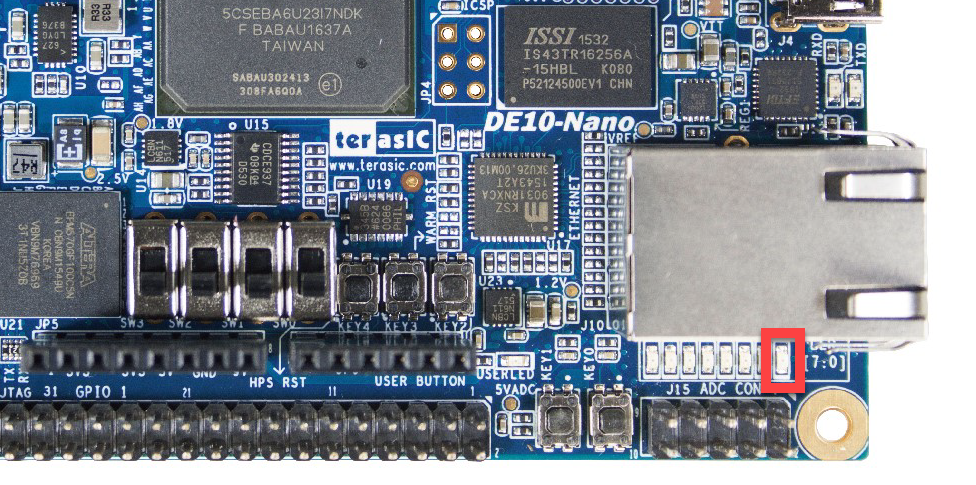
\includegraphics[scale=0.675]{33-blinking-led}
\caption{Blinking LED}
\label{fig:33-blinking-led}
\end{figure}

\end{enumerate}

\end{flushleft}

%----NEW SECTION DEFINITION-----------------------------------------------------
\section*{Experiment on Your Own}
% must manually add TOC reference for unnumbered section
\addcontentsline{toc}{section}{Experiment on Your Own}
%----NEW SECTION DEFINITION-----------------------------------------------------
\begin{flushleft}

\textbf{Change the blink rate}
\newline
\newline
Now that you've got one successful blinking LED under your belt, you can modify the blink rate of the LED by using a different \textquote{bit} of the counter. 1 Hertz is 1 per second (cycles per second) and blinking at 1 Hz means the LED blinks once per second. For 2 Hz, the LED blinks twice per second. And 0.25 Hz would blink the LED once every 4 seconds (slow blink). For a slower blink, use a higher bit of the counter and for faster, use a smaller bit (e.g., cnt[22]). Test out different counter bits and see what you get.

\newpage

\begin{adjustwidth}{2cm}{2cm}
\textit{Clock and Counter Math}
\newline
\newline
\texttt{cnt[n] where n = the counter bit}
\newline
\newline
\texttt{2\^{}n; we've chosen n = 24 in our Verilog code sample}
\newline
\texttt{2\^{}24 = 16,777,216 }
\newline
\newline
Our clock is 50 MHZ or 50,000,000
\newline
\newline
\texttt{Clock / 2\^{}n = blinks per second}
\newline
\texttt{50,000,000 / 16,777,216 = 2.9802}
\newline
\newline
That's about 3 blinks per second.
\newline
\end{adjustwidth}

To make this change, you will need to:

\begin{enumerate}[
	leftmargin=*,
	align=left]

\item Modify the Verilog file (blink.v) and select a different counter bit in the assignment statement.

\item Recompile the design

\item Reprogram the FPGA

\end{enumerate}

\textbf{Add More LEDs}
\newline
\newline
Try connecting one or more of the remaining 7 LEDs to other counter bits, with each blinking at a different rate. For example, you could add a new LED connected to counter bit 23 which would blink twice as fast as bit 24. Or you could add all the remaining 7 LEDs and connect each to a unique counter bit.
\newline
\newline
To make this change, you will need to:

\begin{enumerate}[
	leftmargin=*,
	align=left]

\item Modify the Verilog code:
\begin{enumerate}[
	leftmargin=*,
	align=left]

\item Add the new LEDs to the module definition
\item List the new LEDs as being outputs
\item Assign each of the new LEDs to a unique counter bit (cnt[n])

\end{enumerate}

\emph{I'm new to hardware design. Where can I get the Verilog code that contains these changes?} \hyperlink{side9}{\underline{Sidebar Topic}}

\item Run Analysis and Synthesis

\item Assign the LEDs outputs to pins using the Pin Planner.
\newline
\newline
Be sure to set the proper I/O standard, current strength, and slew rate. The I/O pins connected to the LEDs are as follows:
\newline
\newline
LED[0]: PIN\_W15
\newline
LED[1]: PIN\_AA24
\newline
LED[2]: PIN\_V16
\newline
LED[3]: PIN\_V15
\newline
LED[4]: PIN\_AF26
\newline
LED[5]: PIN\_AE26
\newline
LED[6]: PIN\_Y16
\newline
LED[7]: PIN\_AA23

\item Recompile the design

\item Reprogram the device

\end{enumerate}

\end{flushleft}

%----NEW SECTION DEFINITION-----------------------------------------------------
\section*{Sidebar Topics}
% must manually add TOC reference for unnumbered section
\addcontentsline{toc}{section}{Sidebar Topics}
%----NEW SECTION DEFINITION-----------------------------------------------------
\begin{flushleft}

\hypertarget{side1}{\textbf{Why is the Intel Quartus software download so big?}}
\newline
The Intel Quartus download contains several sophisticated tools to create a custom chip design,  such as simulators, synthesis tools, place and route engines, timing analyzers, and device programmers, to name a few. Nearly all those functions are built into the Intel Quartus Prime Software Suite FPGA design software itself. The download also includes the embedded software design suite for the Nios II soft CPU, and one or more FPGA family databases - in our case the Cyclone V FPGA database.
\newline

\hypertarget{side10}{\textbf{Where should I put my future project files?}}
\newline
Here are a few guidelines you should adopt when choosing a directory for your project:

\begin{itemize}
\item Don't put projects within the Intel Quartus software tool directory. New Intel Quartus software versions come out every six months, so placing them within a specific version directory will make them \textquote{orphans} once a new version is installed. Even worse, you might lose them if you delete the older tool version.
\item Avoid paths with spaces in the name since some of the tools don't like spaces in directory paths.  You might use underscore characters or hyphens instead of space characters in your path names.
\item Use directories where you have read/write access. This sounds intuitive, but sometimes IT departments limit administrator rights. Be sure the folder you create doesn't require admin rights.
\end{itemize}

\hypertarget{side2}{\textbf{What happens during analysis and synthesis?}}
\newline
The Analysis \& Synthesis process:

\begin{itemize}
\item Checks design files for syntax and semantic errors
\item Performs netlist extraction to build a database which integrates all the design files
\item Synthesizes the hardware description language (HDL) code into hardware blocks appropriate for the target FPGA family
\end{itemize}

\hypertarget{side3}{\textbf{What is an SDC file, and why do I need one?}}
\newline
SDC stands for Synopsys Design Constraints and is an industry standard format which defines the timing constraints for a hardware (silicon) design such as the target frequency of the device, and the timing to external peripherals. The SDC file provides a way for the Intel Quartus software to verify that the system generated meets its timing requirements.
\newline
\newline
During synthesis of your FPGA, a design tool called TimeQuest is called by the Intel Quartus software which reads the timing constraints files, calculates the timing of the internal FPGA signals, and compare these timings to the timing requirements specified by the SDC files. A report is created which verifies timing is met and / or identifies signals which fail to meet timing and require optimization.
\newline

\hypertarget{side4}{\textbf{What happens during the fitter (place \& route)?}}
\newline
The fitter places and routes the logic of your synthesized design into target device resources. Think of it like a router that lays out a printed circuit board, connecting the various devices together using copper traces. In this case, however, the devices are logic resources (e.g. lookup tables, registers, memories, multipliers, etc.) and the traces are routing \textquote{wires} inside the FPGA device.
\newline

\hypertarget{side5}{\textbf{What happens during the assembler?}}
\newline
The~assembler generates a programming image from a successful fit which can then be downloaded to the FPGA device.
\newline

\hypertarget{side6}{\textbf{What is timing analysis?}}
\newline
Timing analysis is the process of evaluating the timing of logic in the device after it has been synthesized, placed and routed to ensure the all timing requirements are met. The goal is to achieve \textquote{timing closure} where all the timing constraints are met.
\newline

\hypertarget{side7}{\textbf{Why should I remove the SD Card?}}
\newline
The default behavior of the Terasic DE10-Nano kit is to boot from the SD Card. The processor boots, then configures the FPGA under software control. If you leave the SD Card plugged into the board and then reprogram the FPGA, a watchdog timer in the processor would eventually timeout since the FPGA can no longer respond to the processor because the image has changed. The timeout would force a warm reset which would cause the FPGA to be reprogrammed, overwriting the \textquote{blink} design you just downloaded.
\newline
\newline
This behavior is how the Terasic DE10-Nano kit was designed to operate by default, but is not the way all systems have to behave. You decide how the system responds to warm and cold reset. You may choose to leave the FPGA running \textquote{as is} when a processor reset condition occurs.
\newline

\hypertarget{side8}{\textbf{Why are there two devices found in the JTAG chain?}}
\newline
The Cyclone V SoC device has two JTAG chains, one dedicated to the FPGA and one dedicated to the hard processor system (HPS). As the programmer illustration shows, they are connected in serial on the Terasic DE10-Nano board so you only need one JTAG connection to communicate with both.

\begin{figure}[H]
\centering
% screen shots report a density of 37.8 PixelsPerCentimeter when actual resolution
% is more like 56 PixelsPerCentimeter, so the scaling factor for 1:1 is 0.675
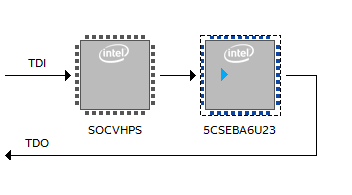
\includegraphics[scale=1.0]{34-sidebar-jtag-chain}
\caption{Terasic DE10-Nano JTAG Chain}
\label{fig:34-sidebar-jtag-chain}
\end{figure}

The FPGA JTAG chain is used to configure the FPGA logic, and for hardware debugging using one of several tools such as:

\begin{itemize}
\item \href{https://www.altera.com/support/training/demonstrations/signaltap-ii.html}{SignalTap II} logic analyzer
\item \href{https://www.altera.com/products/design-software/fpga-design/quartus-prime/features/qts-systems-console.html}{System Console} system-level debugger
\end{itemize}

The HPS JTAG chain is primarily used for software development using tools like the ARM\textsuperscript{*} Development Studio 5\textsuperscript{*} (\href{https://www.altera.com/products/design-software/embedded-software-developers/soc-eds/ds-5-toolkit.html}{DS-5\textsuperscript{*}}).
\newline

\hypertarget{side9}{\textbf{I'm new to hardware design. Where can I get the Verilog code that contains these changes?}}
\newline
Right here:

\begin{minted}[
        bgcolor=MyMintedBGColor,
        fontsize=\small,
        escapeinside=||
]{verilog}

// create module
module blink(
        input  wire       clk,          // 50MHz input clock
        output wire [7:0] LED           // array of 8 LEDs
);


// create a binary counter
reg [31:0] cnt;                         //32 bit counter

initial begin

cnt <= 32'h00000000;                    // start count at zero

end

always @(posedge clk) begin

cnt <= cnt+1;                           // count up

end

//assign LEDs to bits 28 through 21 of the counter

assign LED = cnt[28:21];

endmodule

\end{minted}

\end{flushleft}

\end{document}

